\documentclass{classrep}
\usepackage[utf8x]{inputenc}
\usepackage{color}
\usepackage{environ}
\usepackage{comment}
\usepackage{amsmath}
\usepackage{amssymb}
\usepackage{amsthm}
\usepackage{longtable}
\usepackage{float}
\usepackage{lscape}
\usepackage{icomma}
\usepackage{graphicx}

\newcommand{\card}{\mathrm{card}}
\renewcommand{\labelitemi}{\textbullet}
\renewcommand{\arraystretch}{1.333}

\graphicspath{{graphs}}

\studycycle{Informatyka, studia dzienne, I st.}
\coursesemester{VI}

\coursename{Komputerowe systemy rozpoznawania}
\courseyear{2018/2019}

\courseteacher{dr inż. Marcin Kacprowicz}
\coursegroup{wtorek, 16.15}

\author{
  \studentinfo{Piotr Traczyk}{195733} \and
  \studentinfo{Bartosz Jurczewski}{210209}
}

\title{Zadanie 2: Lingwistyczne podsumowania baz danych}
\svnurl{https://github.com/jurczewski/KSR}

\begin{document}
\maketitle


\section{Cel}
Zadanie polega na stworzeniu aplikacji desktopowej przy użyciu dowolnego formatu bazy danych. W ogólności, aplikacja ma charakter systemu doradczego, który generuje pewną ilość podsumowań lingwistycznych dla podanej bazy, a następnie przedstawia użytkownikowi wybrane – najlepsze wg zastosowanych miar jakości – wyniki, czyli podsumowania lingwistyczne. Aplikacja umożliwiać ma automatyczne generowanie podsumowań lingwistycznych służących do tworzenia krótkich wiadomości tekstowych na podstawie dużej relacyjnej bazy danych. \cite{tresc}


\section{Opis bazy}
Do realizacji zadania wybraliśmy bazę danych \emph{Fifa 19} \cite{data}. Wybrana baza
składa się z \(18128\) krotek znajdujących się w tabeli z \(10\) kolumnami różnych typów. Dane reprezentują piłkarzy w najnowszej odsłonie gry komputerowej Fifa 19.\\ Do tworzenia podsumowań
korzystamy z kolumn:
\begin{enumerate}
    \item Age - wiek
    \item Overall - całkowita ocena zawodnika
    \item Value - wartość zawodnika
    \item Wage - zarobki
    \item Height - wzrost
    \item Weight - waga
    \item FKAccuracy - (free kicks accuracy) - efektywność rzutów wolnych (procent bramek z rzutów wolnych)
    \item SprintSpeed - szybkość w sprincie
    \item Stamina - wytrzymałość
    \item Strength - siła
\end{enumerate}

\begin{figure}[H]
    \centering
    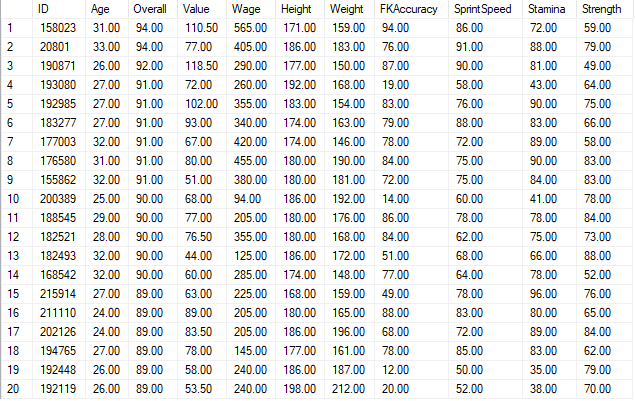
\includegraphics[width=13cm]{/select_baza.png}
    \caption{Fragment widoku tabeli}
\end{figure}
\section{Diagram klas}

\section{Implementacja}
Zaimplementowaliśmy następujące miary. (Wzory zostały wzięte z \cite{adam})
Do obliczania całkowitej miary jakości wykorzystujemy sumę ważoną wszystkich 11 miar. Każda miara ma ustawioną swoją wagę, których suma jest równa 1. T1 ma ustawioną najwyższą wagę równą 7/10, zaś reszta miar taką samą, równą 3/100.

\subsection{Miary jakości podsumowań lingwistycznych}

\subsubsection{\(T_1\) -- stopień prawdziwości}

Najbardziej naturalną miarą jakości podsumowania lingwistycznego
jest wprowadzony przez Yagera stopień prawdziwości.
Abstrahując od tego, czy sumaryzator \(S_j\) jest wynikiem
złożenia wielu sumaryzatorów czy nie, możemy obliczyć
sumę przynależności wszystkich rozważanych krotek do niego:
\[r = \sum_{i=1}^{m} \mu_{\mathrm{ce}(S_j)}(d_i) ~\mbox{,}\]
gdzie \(\mathrm{ce}(S_j)\) jest rozszerzeniem cylindrycznym
sumaryzatora \(S_j\), tak aby otrzymać zbiór rozmyty na uniwersum
możliwych krotek.

Liczbę wszystkich krotek konsekwentnie oznaczamy jako \(m\).
Zatem dla kwantyfikatorów relatywnych stopnień
prawdziwości możemy zapisać jako \(T_1 = \mu_Q(\frac{r}{m})\),
zaś dla kwantyfikatorów absolutnych jako \(T_1 = \mu_Q(r)\).

W przypadku podsumowań z kwalifikatorem wystarczy uwzględnić
przynależność do \(W\) przy liczeniu \(r\), oraz zamiast \(m\)
w mianowniku dla kwantyfikatorów relatywnych zastosować
sumę przynależności wszystkich krotek do \(W\).

\subsubsection{\(T_2\) -- stopień nieprecyzyjności [sumaryzatora]}
Dla podsumowania z \(n\) sumaryzatorami \(S_1 \ldots S_n\)
(w szczególności dla \(n=1\)) możemy określić miarę
jakości podsumowania określaną jako stopień nieprecyzyjności,
definiowaną następującym wzorem:
\[T_2 = 1 - \left(\prod_{j=1}^{n} \mathrm{in}(S_j)\right)^{1/n} ~\mbox{.}\]
Wyrażenie \(\left(\prod_{j=1}^{n} \mathrm{in}(S_j)\right)^{1/n}\) to po prostu
średnia geometryczna ze stopni rozmycia wykorzystanych sumaryzatorów.

\subsubsection{\(T_3\) -- stopień pokrycia}
Miara \(T_3\) dotyczy pewnych własności kwalifikatora,
zatem oczywiście ma sens tylko dla podsumować z kwalifikatorem.
Dla każdego \(i=1\ldots m\) (związanego z krotką \(d_i\) z bazy
danych) możemy zdefiniować:
\[
\begin{array}{l}
t_i = \begin{cases} 1 & \mbox{gdy } \mu_{\mathrm{ce}(S_j)}(d_i) > 0 ~ \wedge ~ \mu_{W}(d_i) > 0 \\
0 & \mbox{w przeciwnym wypadku.}
\end{cases} \\
h_i = \begin{cases}
1 & \mbox{gdy } \mu_{W}(d_i) > 0 \\
0 & \mbox{w przeciwnym wypadku.}
\end{cases}
\end{array}\]

Przy powyższych oznaczeniach:
\[T_3 = \frac{\sum_{i=1}^{m} t_i}{\sum_{i=1}^{m} h_i} ~\mbox{.}\]

\subsubsection{\(T_4\) -- stopień stosowności}
Dla podsumowania z \(n\) sumaryzatorami \(S_1 \ldots S_n\)
oraz \(m\) krotkami w bazie danych możemy wprowadzić oznaczenia:
\[g_{ij} = \begin{cases}
1 & \mbox{gdy } \mu_{\mathrm{ce}(S_j)}(d_i) > 0 \\
0 & \mbox{w przeciwnym wypadku.}
\end{cases}\]
oraz
\[r_j = \frac{\sum_{i=1}^{m} g_{ij}}{m} ~\mbox{.}\]
Wówczas możemy zapisać:
\[T_4 = \left|\left( \prod_{j=1}^{n} r_j \right) - T_3\right| ~\mbox{.}\]

\subsubsection{\(T_5\) -- długość podsumowania}
Dla podsumowania z \(n\) sumaryzatorami \(S_1 \ldots S_n\)
miarę długości podsumowania definiujemy jako:
\[T_5 = 2\left(\frac{1}{2}\right)^{n} ~\mbox{.}\]

\subsubsection{\(T_6\) -- stopień nieprecyzyjności kwantyfikatora}
Nazwy miar \(T_6\)--\(T_{10}\) można określić jako samoopisujące się,
więc przedstawienie wzoru wyczerpuje zagadnienie w stopniu wystarczającym
dla niniejszego sprawozdania:
\[T_6 = 1-\mathrm{in}(Q) ~\mbox{.}\]

\subsubsection{\(T_7\) -- stopień liczności kwantyfikatora}
W przeciwieństwie do \(T_6\), zamiast zliczać elementy z nośnika \(Q\),
policzymy moc zbioru rozmytego:
\[T_7 = 1-\frac{\card(Q)}{\card(\mathcal{X}_Q)} ~\mbox{.}\]

\subsubsection{\(T_8\) -- stopień liczności sumaryzatora}
Możemy mieć do czynienia z sumaryzatorem złożonym; wtedy,
podobnie jak przy poprzednich miarach, stosujemy średnią geometryczną.
Dla podsumowania z \(n\) sumaryzatorami \(S_1 \ldots S_n\):

\[T_8 = 1- \left(\prod_{j=1}^{n} \frac{\card(S_j)}{\card(\mathcal{X}_j)}\right) ~\mbox{.}\]

\subsubsection{\(T_9\) -- stopień nieprecyzyjności kwalifikatora}
Stopień precyzji kwalifikatora \(T_9\) jest oparty na drugiej formie podsumowań tzn.: Q obiektów będących/mających W jest/ma S, gdzie W jest reprezentowane przez zbiór rozmyty i jest kwalifikatorem. Definicja tej miary jest następująca:
\[T_9 = 1-\mathrm{in}(W) ~\mbox{.}\]

\subsubsection{\(T_{10}\) -- stopień liczności kwalifikatora}
Stopień kardynalności kwalifikatora \(T_{10}\) definiujemy jako:
\[T_{10} = 1-\frac{\card(W)}{\card(\mathcal{X}_g)} ~\mbox{.}\]
gdzie miara $\card()$ jest dana tak jak we wcześniejszych sekcjach.


\subsubsection{\(T_{11}\) -- długość kwalifikatora}
Długość kwalifikatora \(T_{11}\) definiujemy następująco:
\[T_{11} = 2\left(\frac{1}{2}\right)^{\card({W})} ~\mbox{.}\]
gdzie $\card(W)$ jest ilością zbiorów rozmytych, z których kwalifikator jest skomponowany. Wniosek jest następujący: im bardziej złożony kwalifikator tym jakość podsumowania gorsza.

\subsection{Funkcje przynależności}
Dla zmiennych lingwistycznych zdefiniowaliśmy następujące funkcje przy-
należności:
\begin{itemize}
    \item{
        [Zbiór rozmyty o trapezoidalnej funkcji przynależności]
        Zbiór rozmyty \(A\) typu I na uniwersum \(\mathbb{R}\) jest
        \emph{liczbą rozmytą trapezoidalną o parametrach \(a, b, c, d\)} wtedy i tylko
        wtedy, gdy \(a \leqslant b \leqslant c \leqslant d\) oraz:
        
        \[\mu_A(x) = \begin{cases}
        0                 & \mbox{gdy } x \leqslant a, \\
        (x - a) / (b - a) & \mbox{gdy } a \leqslant x \leqslant b, \\
        1                 & \mbox{gdy } b \leqslant x \leqslant c, \\
        (d - x) / (d - c) & \mbox{gdy } c \leqslant x \leqslant d, \\
        0                 & \mbox{gdy } d \leqslant x \\
        \end{cases}\]
    }
    \item{
        [Zbiór rozmyty o trójkątnej funkcji przynależności]
        Zbiór rozmyty \(A\) typu I na uniwersum \(\mathbb{R}\) jest
        \emph{liczbą rozmytą trójkątną o parametrach \(a, b, c\)} wtedy i tylko
        wtedy, gdy \(a \leq b \leq c\) oraz:
        
        \[\mu_A(x) = \begin{cases}
        0                 & \mbox{gdy } x \leqslant a, \\
        (x - a) / (b - a) & \mbox{gdy } a \leqslant x \leqslant b, \\
        (c - x) / (c - b) & \mbox{gdy } b \leqslant x \leqslant c, \\
        0                 & \mbox{gdy } c \leqslant x \\
        \end{cases}\]
    }
    \item{Funkcja dyskretna - funkcja dla której wartości dla poszczególnych argumentów określone są z góry}

\end{itemize}

\begin{figure}[H]
    \centering
    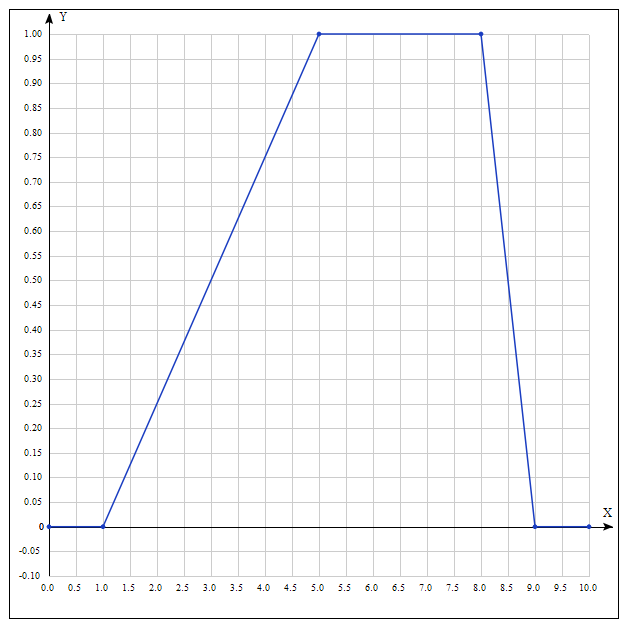
\includegraphics[width=10cm]{/wykres1.png}
    \caption{Wykres funkcji trapezoidalnej dla a=1, b=5, c=9, d=9}
\end{figure}

\begin{figure}[H]
    \centering
    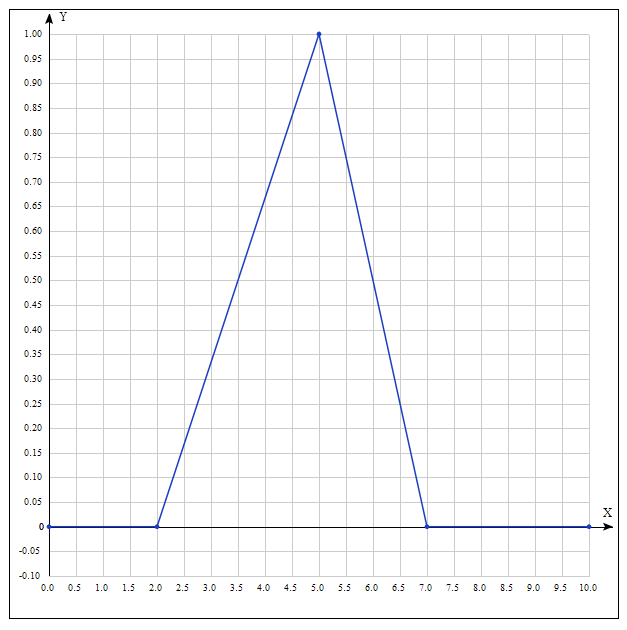
\includegraphics[width=10cm]{/wykres2.png}
    \caption{Wykres funkcji trójkątnej dla a=2, b=5, c=7}
\end{figure}

\subsection{Zmienne lingwistyczne}
W ramach zadania należało stworzyć zmienne lingwistyczne dla kolejnych kolumn bazy danych z etykietami i przyporządkowanymi im zbiorami rozmytymi. Zmienne podzieliliśmy na dwie grupy:
\begin{itemize}
    \item{kwalifikatory i sumaryzatory - używane w programie wymiennie}
    \item{kwantyfikatory}
\end{itemize}

\subsubsection{Kwalifikatory i sumaryzatory}
Poniżej wymienione zostały poszczególne kwalifikatory i sumaryzatory
wedle schematu:
Nazwa zmiennej lingwistycznej - użyta funkcja przynależności A następnie tabela z przyporządkowanymi paramterami funkcji dla poszczególnych etykiet. (Przy funkcjach dyskretnych tabela ma rozpisane przypadki
wartości danych kolumn)
\begin{enumerate}
    \item Age - Funkcja trapezoidalna
    \begin{center}
        \begin{tabular}{|c|c|c|c|c|}
            \hline
            Etykieta & a & b & c & d\\
            \hline
            Young & 8 & 8 & 17 & 20\\
            \hline
            Young Adult & 19 & 23 & 27 & 31\\
            \hline
            Adult & 30 & 35 & 45 & 51\\
            \hline
            Old & 50 & 60 & 90 & 90\\
            \hline
        \end{tabular}
    \end{center}
    \item Overall - Funkcja
    \item Value - Funkcja
    \item Wage - Funkcja
    \item Height - Funkcja
    \item Weight - Funkcja
    \item FKAccuracy - Funkcja
    \item SprintSpeed - Funkcja
    \item Stamina - Funkcja
    \item Strength - Funkcja
\end{enumerate}
\subsubsection{Kwantyfikatory}
Kwalifikatory podzielone są na dwa typy:
\begin{itemize}
    \item{względne}
    \item{bezwzględne}
\end{itemize}
Dla każdego typu została zamieszczona tabela ze stworzonymi etykietami,
funkcjami przynależności oraz ich parametrami ( ”-” oznacza brak danego
parametru)
\begin{enumerate}
    \item{Kwantyfikatory względne}\\
        \begin{center}
        \begin{tabular}{|c|c|c|c|c|c|}
            \hline
            Etykieta & Funkcja & a & b & c & d\\
            \hline
            No & Trójkątna & 0 & 0 & 0.15 & -\\
            \hline
            Less than a third & Trapezoid & 0 & 0 & 0.3 & 0.35\\
            \hline
            Around half & Trójkątna & 0.4 & 0.5 & 0.6 & -\\
            \hline
            Majority & Trójkątna & 0.75 & 0.8 & 0.9 & -\\
            \hline
            All & Trapezoid & 0.85 & 0.9 & 1 & 1\\
            \hline
        \end{tabular}
    \end{center}
    
    \item{Kwantyfikatory bezwzględne}\\
            \begin{center}
        \begin{tabular}{|c|c|c|c|c|c|}
            \hline
                Etykieta & Funkcja & a & b & c & d \\
            \hline
                Less than 5000 & Trapezoid & 0 & 0 & 4990 & 5000 \\
                Around 15000 & Trójkątna & 14000 & 15000 & 16000 & - \\
                Around 25000 & Trójkątna & 24000 & 25000 & 26000 & - \\
                More than 35000 & Trapezoid & 35000 & 35010 & 41000 & 41000 \\
            \hline
        \end{tabular}
    \end{center}

    
    
    
\end{enumerate}


\section{Interfejs użytkownika}

\section{Dyskusja}

\section{Wnioski}
\begin{itemize}
\item Podsumowania lingwistyczne są bardzo dobrą 
\end{itemize}

\begin{thebibliography}{}
  \bibitem{tresc}
    A. Niewiadomski,
    \emph{Komputerowe Systemy Rozpoznawania: Materiały, przykłady i ćwiczenia do przedmiotu}.
    21 września 2009.
    http://ics.p.lodz.pl/~aniewiadomski/ksr/ksr-projekt2.pdf
    \bibitem{data}
    Baza danych - "FIFA 19 complete player dataset":\\
    \url{https://www.kaggle.com/karangadiya/fifa19}    
  \bibitem{zadeh}
    L. A. Zadeh,
    \emph{A fuzzy-set-theoretical interpretation of linguistic hedges}.
    Journal of Cybernetics 1972; 2: 4–34.
  \bibitem{adam}
    A. Niewiadomski,
    \emph{Methods for the Linguistic Summarization of Data: Applications of Fuzzy Sets and Their Extensions}.
    Akademicka Oficyna Wydawnicza EXIT,
    Warszawa 2008.
    
\end{thebibliography}
\end{document}
